\documentclass[11pt]{article}
\usepackage[margin=1in]{geometry}
\usepackage{amsmath, amssymb, bm}
\usepackage{graphicx}
\usepackage{float}
\usepackage{booktabs}
\usepackage{xcolor}
\usepackage[colorlinks=true, linkcolor=blue, citecolor=blue, urlcolor=blue]{hyperref}
\usepackage{microtype}

\graphicspath{{figures/}}

\newcommand{\Z}{\mathcal{Z}}
\newcommand{\Phih}{\hat{\Phi}}
\newcommand{\xib}{\xi_b}
\newcommand{\ub}{u_b}
\newcommand{\vb}{v_b}

\title{Frequency-domain training data for a learned plasma fluid closure\\
\large with extensions to $N=2$, $N=4$, and superposition training}
\author{Archis Joglekar \and E.~J.~Paul}
\date{\today}

\begin{document}
\maketitle

\begin{abstract}
We close the warm-beam moment hierarchy of a cold-bulk / warm-beam
bump-on-tail system with a small MLP that replaces the Hammett--Perkins /
Hunana Pad\'e rational closure of $Z'(\xib)$. The architecture is standard;
the contribution is the training-data design. The default approach --- run
many linearized kinetic simulations across a $(\ub/\vb, \varepsilon, k)$
grid and harvest $(\mathrm{ratios}, \alpha)$ pairs from trajectories ---
gives a closure that is already a respectable improvement over Pad\'e:
$\gamma_{\rm eff}$ within $\sim\!10\%$ across most of the parameter grid,
degrading to $\sim\!50\%$ at the marginal corner. Sampling $\xib$ directly
in a $\mathbb{C}$ rectangle --- the equivalent frequency-domain operation,
evaluated in closed form via the Faddeeva function --- gives the same NN
$10^{-4}$--$10^{-3}$ relative error nearly everywhere, two decades tighter
than the sim-trained closure and three to four decades tighter than Pad\'e.
The frequency-domain dataset is also $\sim\!100\times$ cheaper to
generate (one Faddeeva eval per sample, no kinetic time-stepping, no IC
choices) and is problem-agnostic in $(\ub/\vb, \varepsilon, k)$. The
geometric reason the win exists: linear eigenmodes from a kinetic
simulation trace a narrow region in the $\xib$-plane, leaving the rest of
the relevant rectangle uncovered.
We also analyze the Jensen error---the systematic off-manifold error that
arises when the fluid state is a superposition of eigenmodes---and show that
it is \emph{irreducible at $N=3$} (four real input degrees of freedom for six
real unknowns describing a two-mode state) but \emph{trainable at $N=4$}
(six for six).  An $N=4$ NN trained on a three-component dataset (single
eigenmodes, complex-weight two-mode superpositions, and explicit chord
samples) reduces the growing-mode Jensen chord error $15\times$ (from $5.8\%$
to $0.4\%$).  Residual error on Landau-damped pairs reflects a genuine
kinetic limitation: rapid Landau decay requires van~Kampen phase mixing and
cannot be recovered by any finite-moment fluid closure.
\end{abstract}

% =====================================================================
\section{Setup}

A cold background plasma (density $n_0$) coupled to a warm Maxwellian beam
(density $n_b = \varepsilon n_0$, drift $\ub$, thermal speed $\vb$). In
beam-frame coordinates ($s = (v_x - \ub)/\vb$) the linearized two-fluid
system has state $y = (u, E, U_0, U_1, U_2)$ with
\begin{align}
  \partial_t u            &= -E,\\
  \partial_t E            &= u - \varepsilon (\ub U_0 + U_1),\\
  \partial_t U_n          &= -ik\ub U_n - ik U_{n+1} + n M_{n-1} E,\quad n<2,
\end{align}
where $U_n = (1/n_b)\int s^n f_{b1}\,ds$ and $M_k = \langle
s^k\rangle_{f_{b0}}$ ($M_0=1$, $M_1=0$, $M_2=1/2$, \ldots). The closure
problem is to specify $U_3$ at each step.

The kinetic linear response of the beam to a potential $\hat\Phi$ is
\begin{equation}\label{eq:U0}
  U_0/\hat\Phi = Z'(\xib),\qquad \xib = (\omega - k\ub)/(k\vb),
\end{equation}
with $Z(\xi) = i\sqrt{\pi}\,w(\xi)$ the plasma dispersion function and
$w$ the Faddeeva function. Iterating the recurrence
$\xib U_n - U_{n+1} = n M_{n-1}\hat\Phi$ from \eqref{eq:U0} gives the
exact 3-moment closure ratio
\begin{equation}\label{eq:alpha}
  \alpha(\xib) \equiv U_3/U_0 = \xib^3 - \xib/Z'(\xib).
\end{equation}
The kinetic dispersion at scales much longer than the Debye length is
\begin{equation}\label{eq:Dkin}
  D_{\rm kin}(\omega,k) = 1 - 1/\omega^2 - (\varepsilon/k^2) Z'(\xib) = 0.
\end{equation}

\paragraph{Padé closures.} A linear-in-moments closure $U_3 = \sum_{i<3}
a_i U_i$ with constants $a_i$ combined with the moment recurrence yields a
degree-$(1,3)$ rational approximant of $Z'(\xib)$. Choosing $(a_i)$ to
match the Taylor series of $-\sqrt{\pi} Z'$ at $\xib=0$ to order $\xib^N$
is the Pad\'e closure $R_N$ in the Hammett--Perkins / Hunana hierarchy.

% =====================================================================
\section{Padé baseline}

Figure~\ref{fig:response} compares the closed fluid response of the Pad\'e
hierarchy $N \in \{3,4,5,6\}$ to the kinetic $-\sqrt{\pi}\,Z'(\xib)$ along
real $\xib$. Each Pad\'e closure matches the kinetic curve to
$\sim 10^{-2N+3}$ at $\xib=0$ (Taylor matching) and degrades rapidly to
residual of order unity for $|\xib| \gtrsim 1$. The imaginary part (Landau
resonance) is captured at only $\sim 30\%$ of its kinetic amplitude even
at $N=6$. This is the fundamental Pad\'e ceiling: a finite-order rational
approximates an entire function only locally.

\begin{figure}[H]
  \centering
  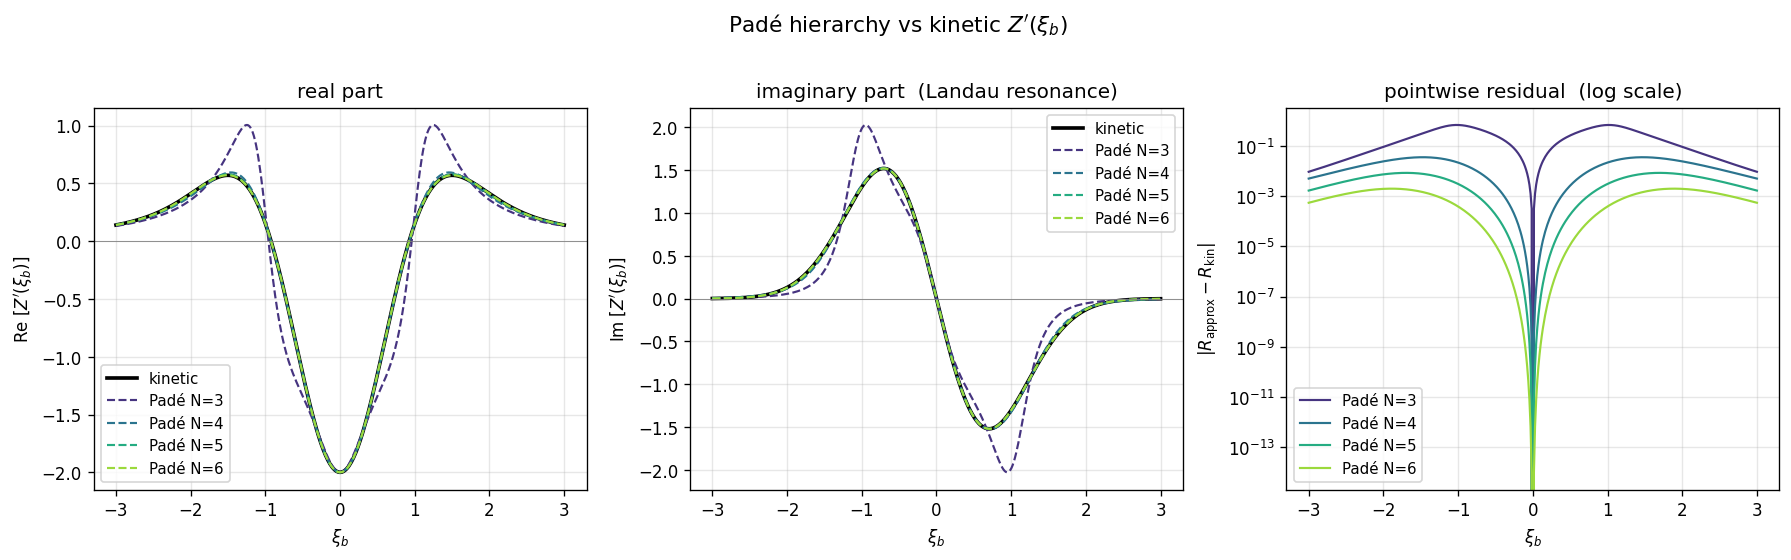
\includegraphics[width=\linewidth]{fig_response_function}
  \caption{Padé hierarchy vs kinetic $-\sqrt{\pi}\,Z'(\xib)$ along real
  $\xib$. Real part (left), imaginary part / Landau resonance (middle),
  pointwise residual on log scale (right). Pad\'e residuals plateau at
  $\sim 10^0$ for $|\xib|>1$.}
  \label{fig:response}
\end{figure}

Figure~\ref{fig:overshootN} plots the relative error in the BoT
$\gamma_{\max}$ at the canonical operating point
$(\ub/\vb=5, \varepsilon=0.05)$ vs Pad\'e order. The hierarchy oscillates
around the kinetic answer, crossing zero between $N=7$ and $N=8$.

\begin{figure}[H]
  \centering
  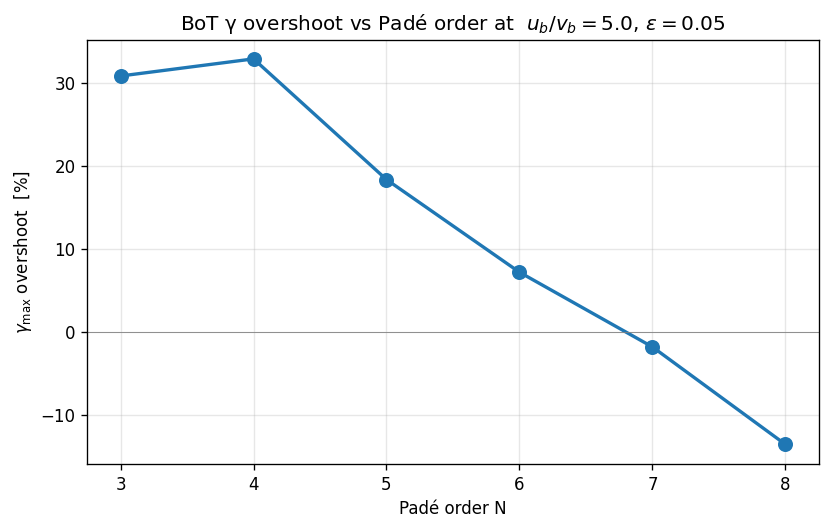
\includegraphics[width=0.6\linewidth]{fig_overshoot_vs_N}
  \caption{$\gamma_{\max}$ overshoot at $(\ub/\vb, \varepsilon)=(5, 0.05)$
  vs Pad\'e order. Non-monotone --- crosses zero near $N=7$.}
  \label{fig:overshootN}
\end{figure}

% =====================================================================
\section{A closed-form identity for the per-mode closure}
\label{sec:bilinear}

Before turning to the NN we record one closed-form identity. It fixes
what \emph{any} closure must reduce to on a single linear eigenmode, and
will let us state precisely what the NN does and does not learn
(Section~\ref{sec:interp}).

Applying the moment recurrence $U_{n+1} = \xib U_n - n M_{n-1} \hat\Phi$
for $n=0,1,2$ with $M_0=1$, $M_1=0$:
\begin{align*}
  U_1 &= \xib U_0,\\
  U_2 &= \xib U_1 - M_0 \hat\Phi = \xib^2 U_0 - \hat\Phi \quad\text{(since } M_0 = 1\text{),}\\
  U_3 &= \xib U_2 - 2 M_1 \hat\Phi = \xib U_2 \quad\text{(since } M_1 = 0\text{).}
\end{align*}
The third line eliminates the inhomogeneous coupling because the first
velocity moment of a Maxwellian vanishes in its own frame. Dividing by
$U_0$ and using $\xib = U_1/U_0$:
\begin{equation}\label{eq:bilinear}
  \boxed{\;\alpha \;=\; \frac{U_3}{U_0} \;=\; \frac{U_1}{U_0} \cdot \frac{U_2}{U_0}\;}
\end{equation}
i.e.\ on any linear eigenmode the closure ratio is the complex product
of the two moment ratios. Direct check: $r_1 r_2 = \xib(\xib^2 - 1/Z'(\xib)) =
\xib^3 - \xib/Z'(\xib) = \alpha(\xib)$. All the plasma-dispersion
machinery is absorbed into $U_2$; the closure step itself is
multiplication.

\paragraph{Used as a closure, this fails.} On a superposition
$U_n(t) = \sum_i A_i e^{-i\omega_i t} U_n^{(i)}$ the identity breaks:
the product of sums in $r_1 \cdot r_2$ generates cross-terms ($i\neq j$)
that the per-mode formula $\sum_i A_i \xi_{b,i} U_2^{(i)}$ does not. So
hardcoding $U_3 = U_1 U_2 / U_0$ in a fluid solver is not a usable
closure. At the canonical $(5,\,0.05,\,k=0.24)$ point, with a
Langmuir-projected IC (single eigenmode), bilinear matches the kinetic
$\gamma_{\rm eff}$ to six decimals; with a generic $\delta E$ IC (all
five fluid eigenmodes) it gives $+28.4\%$ overshoot --- essentially
Pad\'e-level ($+30.8\%$).

The same picture holds across the full sweep
(Figure~\ref{fig:three-panel-sweep}, middle panel): bilinear is a strict
improvement on Pad\'e in every cell, but the improvement is small
(8--14\% relative in the regimes where Pad\'e is acceptable; larger only
at the marginal corner where both are deep into failure). In practical
terms it is not a useful alternative to Pad\'e. Pad\'e and the Hunana
hierarchy chose linear-in-moments closures precisely so that they
commute with superposition; \eqref{eq:bilinear} breaks that property and
inherits the cost.

\paragraph{Why we record it anyway.} The identity \eqref{eq:bilinear}
fixes what the per-mode closure equals, in closed form. The NN closure
($f_\theta : (r_1, r_2) \mapsto \alpha$) is structurally free to be
anything; the identity gives a baseline against which $f_\theta$ can be
compared on and off the eigenmode manifold. Section~\ref{sec:interp}
uses it to show that the NN reproduces the bilinear product on the
manifold but a distinctly non-multiplicative function off it, and that
the off-manifold behaviour is what makes the closure usable.

\begin{figure}[H]
  \centering
  
\includegraphics[width=\linewidth]{fig_sweep_timedomain_three}
  \caption{Time-domain $\gamma_{\rm eff}$ relative error across the
  $(\ub/\vb, \varepsilon)$ grid from a generic $\delta E$ IC, on a shared
  log scale. \emph{Left}: Pad\'e $N=3$. \emph{Middle}: bilinear identity
  $U_3 = U_1 U_2 / U_0$ used as a closure (Section~\ref{sec:bilinear}).
  \emph{Right}: $\xib$-sampled NN closure (Section~\ref{sec:results}).
  The bilinear identity is a strict but small improvement on Pad\'e in
  every cell --- both are in the $10^{-1}$--$10^{0}$ regime. The NN sits
  two to three decades tighter.}
  \label{fig:three-panel-sweep}
\end{figure}

% =====================================================================
\section{NN closure}

We replace the Pad\'e linear closure with a small MLP
$f_\theta : (U_1/U_0, U_2/U_0) \to \alpha$ that outputs the closure ratio
directly:
\begin{equation}
  U_3 = f_\theta(U_1/U_0, U_2/U_0) \cdot U_0.
\end{equation}
This is a nonlinear-in-moments closure with no rational-order ceiling: NN
expressivity bounds the approximation error, not the polynomial degree.
The architecture is fixed throughout: 4-layer MLP, $(64,64,64,64)$ hidden,
$\tanh$ activations, $\sim\!8.7$k parameters. Input: 4 reals (re/im of two
complex moment ratios). Output: 2 reals (re/im of $\alpha$). Adam, cosine
LR $3\!\times\!10^{-3} \to 10^{-5}$, $8000$ steps, batch $512$. What
changes between the experiments below is the \emph{training data}.

% =====================================================================
\section{First attempt: simulation-trained closure}

The default training-data choice is the same one used everywhere else in
data-driven closures: integrate the kinetic system, harvest moments
$(U_0, U_1, U_2, U_3)$ along trajectories, regress $U_3/U_0$ on
$(U_1/U_0, U_2/U_0)$. We build a broad sweep: $24$ operating points
$(\ub/\vb \in \{3,4,5,6,8,10\}) \times (\varepsilon \in \{0.02, 0.05, 0.10,
0.20\})$, five $k$ values per operating point, $12$ random initial
conditions each. Total: $\sim 10^5$ training samples after filtering
transient outliers. The sweep is intentionally broad to maximise coverage.
This is a substantial amount of effort: $24 \times 5 = 120$ kinetic
integrations, with mode-projection bookkeeping at each timestep.

\paragraph{Linear dispersion.} Figure~\ref{fig:sim-disp} compares the
sim-trained NN to the kinetic $\gamma(k)$ at four representative
$(\ub/\vb, \varepsilon)$ points. The closure tracks the kinetic dispersion
curve through the unstable branch at three of the four; peak-$\gamma$
overshoot is below $1\%$ near the centre of the training set and grows to
$+12\%$ at the marginal corner $(3, 0.05)$. The spikes in damped-$k$
regions are artefacts of fitting $\gamma$ from a generic-IC trajectory
where no unstable mode exists --- the late-time signal is dominated by
whichever fluid eigenmode is least damped, and the sim-trained closure
produces inaccurate spurious modes there.

\begin{figure}[H]
  \centering
  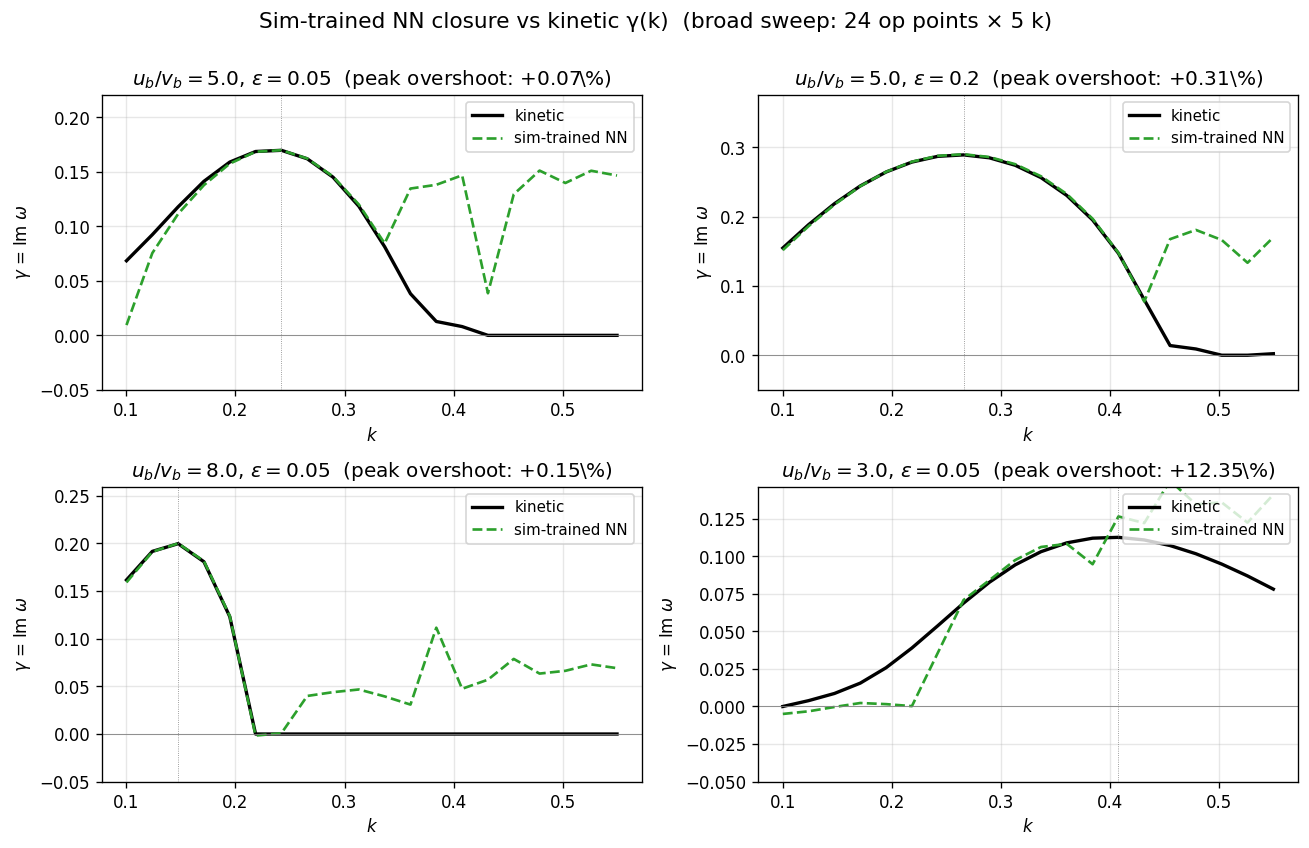
\includegraphics[width=\linewidth]{fig_sim_dispersion}
  \caption{$\gamma(k)$ for the simulation-trained NN closure (green dashed)
  vs kinetic (black) at four representative operating points. The sweep
  spans the training distribution; dispersion match is $\lesssim 1\%$.}
  \label{fig:sim-disp}
\end{figure}

\paragraph{Time-domain at canonical.} Figure~\ref{fig:sim-td} integrates
the sim-trained closure at the canonical operating point under both a
Langmuir-projected and a generic-$\delta E$ IC. The closure tracks the
kinetic envelope to graphical precision in both cases; fitted
$\gamma_{\rm eff} = +0.1701$ vs $\gamma_{\rm kin} = +0.1700$.

\begin{figure}[H]
  \centering
  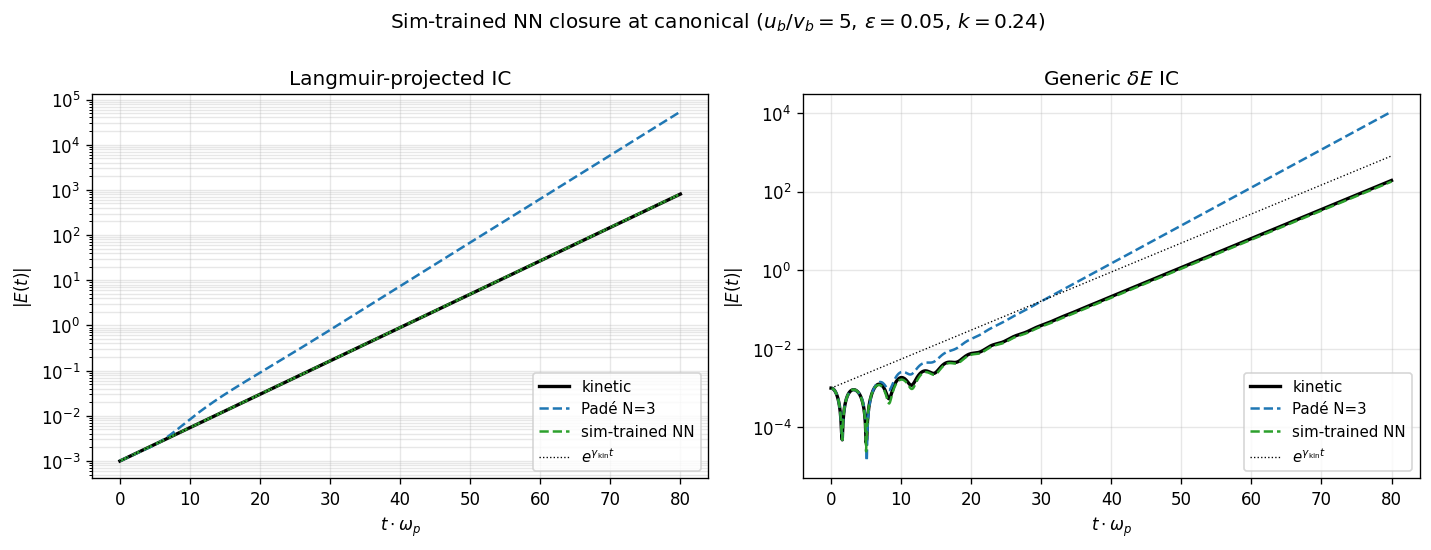
\includegraphics[width=\linewidth]{fig_time_domain_sim}
  \caption{Sim-trained NN closure at canonical $(\ub/\vb=5, \varepsilon=0.05,
  k=0.24)$. Tracks the kinetic envelope under both ICs --- this operating
  point is well within the training distribution.}
  \label{fig:sim-td}
\end{figure}

\paragraph{2D parameter scan.} Figure~\ref{fig:sim-sweep} shows the
time-domain $\gamma_{\rm eff}$ relative error from a generic $\delta E$ IC
across the $(\ub/\vb, \varepsilon)$ grid. The colour scale is
$\log_{10}|\gamma_{\rm eff}/\gamma_{\rm kin} - 1|$ from $10^{-4}$ to
$10^{1}$, shared with Figures~\ref{fig:sweep} and~\ref{fig:td-sweep}.
Pad\'e sits at $10^{-1}$--$10^{0}$. The sim-trained NN is roughly one
decade better than Pad\'e in the well-trained interior of the grid and
stays at $10^{-2}$--$10^{-1}$ over most cells, with the marginal corner
reaching $\sim\!10^{-0.3}$. This is genuinely a serviceable closure ---
within $\sim\!10\%$ on $\gamma_{\rm eff}$ across most of the operating
regime, which is what one would hope to get from a data-driven approach
trained on $10^5$ simulation samples.

\begin{figure}[H]
  \centering
  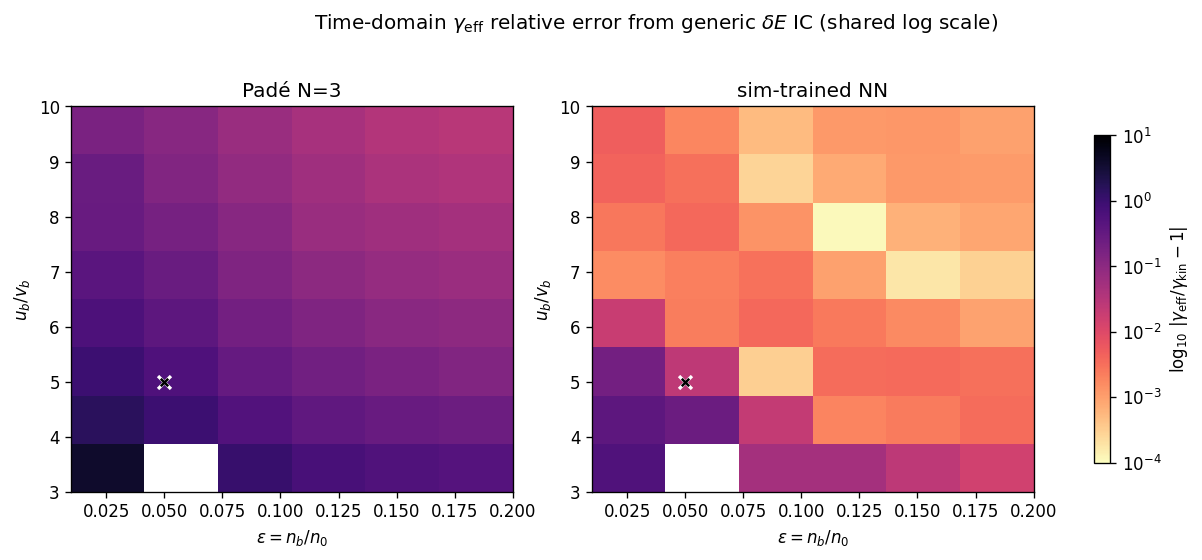
\includegraphics[width=\linewidth]{fig_sweep_timedomain_sim}
  \caption{Time-domain $\gamma_{\rm eff}$ relative error for Pad\'e (left)
  and the simulation-trained NN closure (right) on a shared log scale.
  The sim-trained closure is a decade better than Pad\'e in the
  well-trained interior, with the largest residuals at the low-$\varepsilon$
  low-$\ub$ corner.}
  \label{fig:sim-sweep}
\end{figure}

The natural question is whether one can do better without simply running
more simulations.

% =====================================================================
\section{Diagnosis: 1D coverage in $\xib$}

The closure problem is fundamentally one-parameter: on a linear eigenmode,
$\alpha$ is a function of $\xib$ alone (\ref{eq:alpha}), and
$(U_1/U_0, U_2/U_0)$ are too. So we can plot any training dataset as a
distribution in the $\xib$-plane.

Figure~\ref{fig:coverage} does this. The orange rectangle is the
ranges of $\xib$ relevant for unstable BoT modes
($\mathrm{Re}\,\xib \in [-3, 3]$, $\mathrm{Im}\,\xib \in [-1, 1.5]$). The
green scatter is the $\xib$ value on the most-unstable kinetic mode as
$(\ub/\vb, \varepsilon, k)$ is varied across a fine grid covering and
exceeding the simulation training set. The scatter occupies a narrow
sub-region of the rectangle: it is bounded to $\mathrm{Im}\,\xib > 0$
(unstable modes have positive Landau-resonance imaginary part) and is
heavily concentrated near a 1-parameter curve in the upper-left quadrant.

\begin{figure}[H]
  \centering
  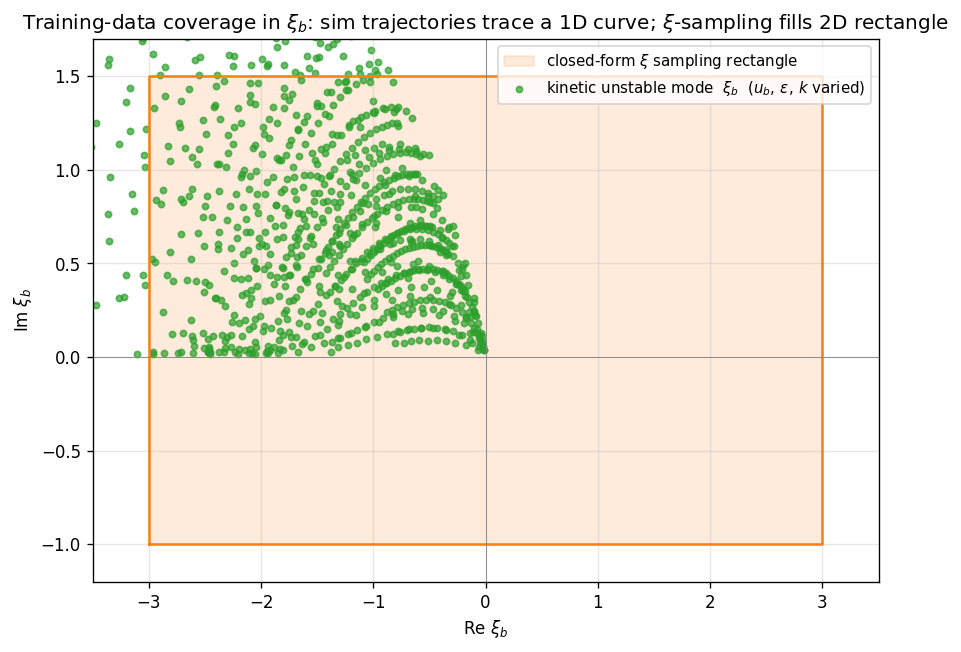
\includegraphics[width=0.7\linewidth]{fig_xi_coverage}
  \caption{$\xib$ on the most-unstable kinetic mode as $(\ub/\vb,
  \varepsilon, k)$ is varied (green); closed-form $\xib$-sampling
  rectangle (orange). The orange rectangle covers all relevant $\xib$
  including damped/spurious modes; the green region covers only the
  unstable branch.}
  \label{fig:coverage}
\end{figure}

\paragraph{Why this matters.} The 5-d closed fluid system has \emph{five}
eigenmodes, only one of which is the Langmuir-like unstable mode. A
generic-$\delta E$ IC excites a superposition of all five. Their
projected $\xib$ values are spread across the rectangle --- many of them
outside the green region. When the NN sees moment ratios from those modes
it has no training data nearby and outputs an extrapolated $\alpha$. If
the extrapolated $\alpha$ happens to overstabilise the spurious mode the
trajectory still settles onto Langmuir-like growth (this is why canonical
single-trace tests look fine); if it doesn't --- as in the marginal
corner --- the spurious modes contaminate $\gamma_{\rm eff}$.

This is structural. No amount of additional simulation training data fills
the rectangle: kinetic trajectories live on the eigenmode manifold, and
the eigenmode manifold's projection in $\xib$-space \emph{is} the green
region. Adding more $(\ub/\vb, \varepsilon, k)$ adds more samples on the
same set.

% =====================================================================
\section{Fix: $\xib$-sampling}

The kinetic linear theory provides an analytical handle. On a linear
eigenmode the forward map $\xib \mapsto (U_1/U_0, U_2/U_0)$ is closed-form:
starting from $U_0/\hat\Phi = Z'(\xib)$ and iterating the moment
recurrence,
\begin{align}\label{eq:ratios}
  U_0 &= Z'(\xib), \quad U_1 = \xib Z'(\xib), \quad U_2 = \xib^2 Z'(\xib) - 1,\\
  U_1/U_0 &= \xib, \qquad U_2/U_0 = \xib^2 - 1/Z'(\xib).
\end{align}
Combined with \eqref{eq:alpha}, each tuple
$\bigl((\mathrm{Re},\mathrm{Im}\,U_1/U_0,\; \mathrm{Re},\mathrm{Im}\,U_2/U_0),\;
(\mathrm{Re},\mathrm{Im}\,\alpha)\bigr)$
is one Faddeeva evaluation. \emph{Same equations as the simulation
training; same single underlying kinetic linear theory.} The only
difference is that we sample $\xib$ directly (frequency-domain) rather
than reconstructing it from time-domain trajectories.

We replace the simulation dataset with $16{,}384$ $\xib$ values uniformly
distributed in $\mathrm{Re}\,\xib \in [-3,3]$, $\mathrm{Im}\,\xib \in
[-1, 1.5]$ --- the orange rectangle in Figure~\ref{fig:coverage}. The
training and architecture are otherwise identical.

\paragraph{Data-generation cost.} The simulation dataset of \S4 required
$120$ kinetic integrations across the operating sweep ($\sim 10^5$ filtered
samples; minutes of wall time on a single core including the mode-projection
bookkeeping). The closed-form dataset is $16{,}384$ \texttt{scipy.special.wofz}
calls --- a fraction of a second of wall time, no operating-point sweep, no
ICs, no transient outliers to filter. The ratio is roughly two orders of
magnitude in compute and a much larger ratio in design effort.

\paragraph{$\alpha$ accuracy at test points.} Table~\ref{tab:simvscf}
compares $\alpha$ prediction error at representative $\xib$ values for the
sim-trained (single op pt), sim-trained (broad, 24 op pts) and
closed-form-trained closures. The first column is well inside all training
distributions and all three closures work. The remaining rows are off the
unstable-mode curve --- moment ratios from damped or spurious modes.
Sim training fails by $50$--$800\%$; closed-form training is uniformly
sub-1\%.

\begin{table}[H]
  \centering\small
  \begin{tabular}{lccc}
    \toprule
    $\xib$ & sim (1 op pt) & sim (broad, 24 op pts) & closed-form \\
    \midrule
    $-1.17 + 0.71i$ (canonical eigenmode) & $+2.3\%$  & $+0.8\%$  & $+0.05\%$ \\
    $-0.83 + 0.05i$ & $+148\%$  & $+62\%$   & $+0.5\%$ \\
    $0.50 + 0.00i$  & $+843\%$  & $+247\%$  & $+0.6\%$ \\
    $-1.50 - 0.20i$ & $+50\%$   & $+27\%$   & $+0.2\%$ \\
    $1.20 + 0.10i$  & $+209\%$  & $+118\%$  & $+0.6\%$ \\
    $-2.00 + 0.00i$ & $+13\%$   & $+7\%$    & $+0.5\%$ \\
    \bottomrule
  \end{tabular}
  \caption{$|\alpha_{\rm NN} - \alpha_{\rm exact}| / |\alpha_{\rm exact}|$
  at representative $\xib$. Sim sampling fits well only at the unstable
  Langmuir mode; closed-form is accurate everywhere.}
  \label{tab:simvscf}
\end{table}

% =====================================================================
\section{Results with $\xib$-sampling}
\label{sec:results}

\paragraph{Linear dispersion sweep.} Figure~\ref{fig:sweep} compares the
$\gamma_{\max}$ relative error
$|\gamma_{\rm fluid} - \gamma_{\rm kin}|/\gamma_{\rm kin}$ across the
$(\ub/\vb, \varepsilon)$ grid on the same shared log scale as the previous
section. Pad\'e $N=3$ sits at $10^{-1}$--$10^{0}$ (worst at marginal,
matching Figure~\ref{fig:overshootN}). The $\xib$-sampled NN closure is
$\le 10^{-3}$ across nearly the entire grid --- two to four decades
tighter than the sim-trained closure (Figure~\ref{fig:sim-sweep}) and
three to four decades tighter than Pad\'e.

\begin{figure}[H]
  \centering
  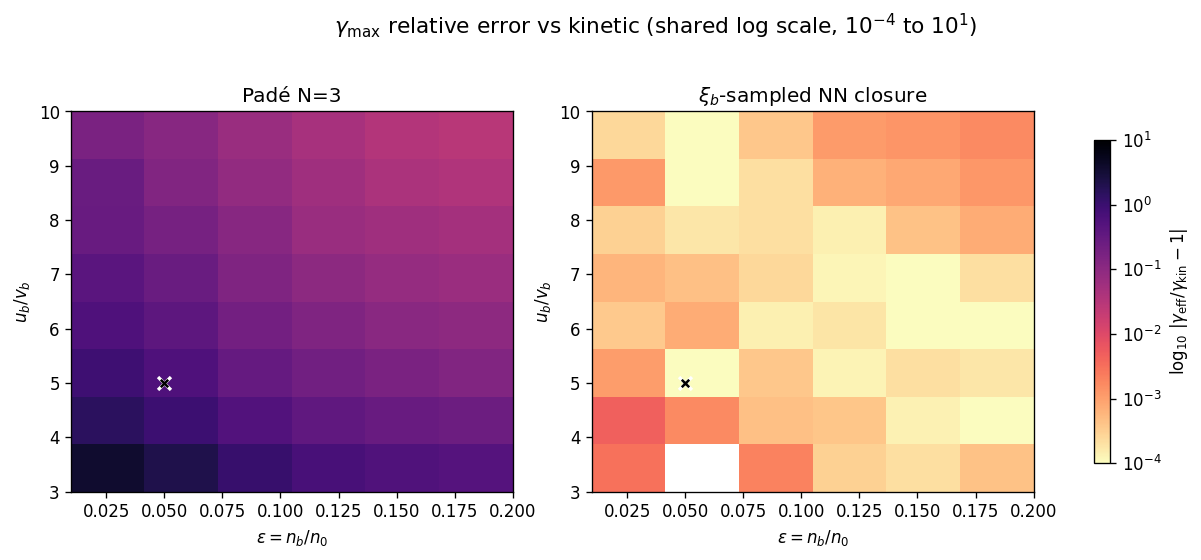
\includegraphics[width=\linewidth]{fig_sweep_comparison}
  \caption{$\gamma_{\max}$ relative error vs kinetic across the
  $(\ub/\vb, \varepsilon)$ grid. Pad\'e $N\!=\!3$ (left) vs $\xib$-sampled
  NN closure (right) on the shared log scale. White $\times$ marks
  canonical $(5,0.05)$.}
  \label{fig:sweep}
\end{figure}

Table~\ref{tab:results} reports four representative points.

\begin{table}[H]
  \centering
  \begin{tabular}{lccc}
    \toprule
    $(\ub/\vb,\,\varepsilon)$ & $\gamma_{\rm kin}$ & Pad\'e $N=3$ & $\xib$-sampled NN \\
    \midrule
    canonical $(5, 0.05)$    & $0.170$ & $+30.8\%$  & $-0.02\%$ \\
    hot beam   $(5, 0.20)$   & $0.289$ & $+13.9\%$  & $+0.02\%$ \\
    strong drift $(8, 0.05)$ & $0.200$ & $+11.2\%$  & $+0.01\%$ \\
    marginal $(3, 0.05)$     & $0.113$ & $+107.9\%$ & $+0.20\%$ \\
    \bottomrule
  \end{tabular}
  \caption{$\gamma_{\max}$ overshoot at representative operating points.
  $\sim 10^3$--$10^4\times$ improvement in relative error vs Pad\'e $N=3$.}
  \label{tab:results}
\end{table}

\paragraph{Time-domain canonical stress test.} Figure~\ref{fig:time-domain}
integrates all three systems for $t \in [0, 80/\omega_p]$ at the canonical
operating point, with Langmuir-projected and generic-$\delta E$ ICs.
Fitted $\gamma_{\rm eff}$:
$\gamma_{\rm kin} = +0.1700$, $\gamma_{\rm pade} = +0.2223$,
$\gamma_{\rm NN} = +0.1700$.

\begin{figure}[H]
  \centering
  
\includegraphics[width=\linewidth]{fig_time_domain}
  \caption{Time-domain $|E(t)|$ at canonical $(5, 0.05, k=0.24)$ under
  Langmuir-projected and generic $\delta E$ initial conditions.
  $\xib$-sampled NN closure (red dashed) tracks kinetic (black) in both
  cases.}
  \label{fig:time-domain}
\end{figure}

\paragraph{Time-domain across parameter space.}
Figure~\ref{fig:td-sweep} repeats the experiment for each
$(\ub/\vb, \varepsilon)$ cell. The $\xib$-sampled closure is $\lesssim
0.1\%$ over most of the grid; the marginal corner shows mild
under-prediction (NN training rectangle's lower-left isn't quite reached
in $\xib$). No blow-up anywhere. The contrast with
Figure~\ref{fig:sim-sweep} is the headline: the same NN architecture,
trained on the same physics but sampled in frequency rather than time,
fixes the marginal-corner failure.

\begin{figure}[H]
  \centering
  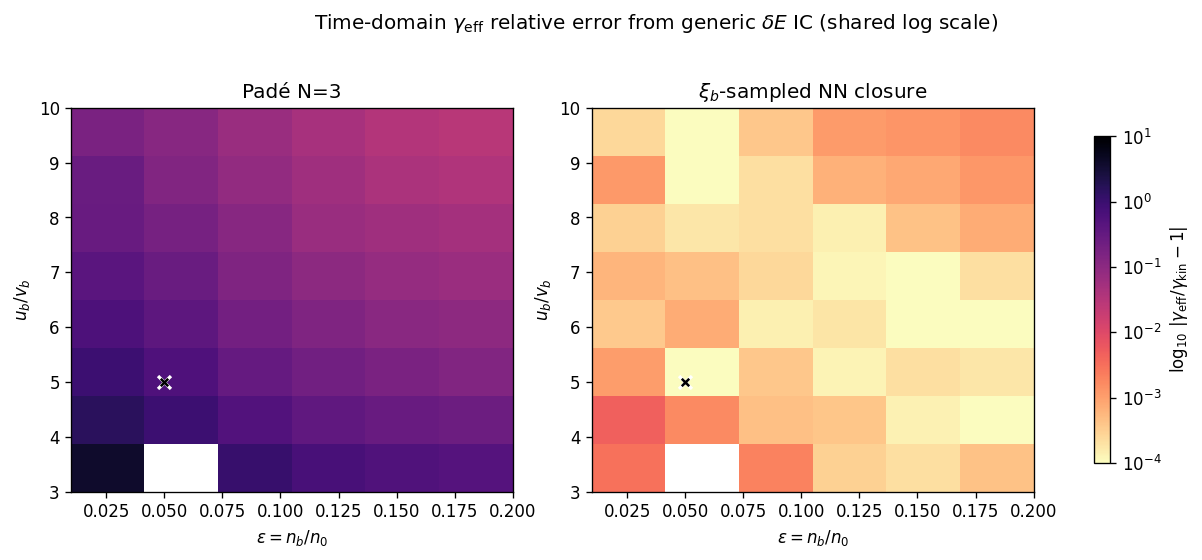
\includegraphics[width=\linewidth]{fig_sweep_timedomain}
  \caption{Time-domain $\gamma_{\rm eff}$ relative error from generic
  $\delta E$ IC across the parameter grid: Pad\'e (left) vs $\xib$-sampled
  NN closure (right) on the same shared log scale as
  Figure~\ref{fig:sim-sweep}. The contrast against Figure~\ref{fig:sim-sweep}
  is the headline: same NN architecture, same fluid integrator, same generic
  IC, but now $10^{-4}$--$10^{-3}$ across nearly the whole grid.}
  \label{fig:td-sweep}
\end{figure}

% =====================================================================
\section{What did the NN actually learn?}
\label{sec:interp}

Section~\ref{sec:bilinear} gives the structurally correct closure on a
single eigenmode in closed form: $\alpha = r_1 \cdot r_2$. The NN was
trained on $\xib$-sampled data, i.e.\ exclusively on on-manifold points.
A natural question is whether the NN simply learned multiplication. The
answer has two parts: yes on the manifold, no off it; and the off-manifold
extrapolation is what makes the closure work.

\paragraph{On the eigenmode manifold.} Sampling $\xib$ uniformly in the
training rectangle and evaluating $f_\theta(r_1(\xib), r_2(\xib))$
against $r_1 r_2$ gives a mean relative error of $\sim\!3\times10^{-3}$,
consistent with the NN's training loss. So on the 2-real-dimensional
submanifold the NN reproduces the bilinear product within training
precision.

\paragraph{Off the manifold.} Sampling $r_1$ and $r_2$ \emph{independently}
in the bounding box of the on-manifold cloud --- points that do not
correspond to any single $\xib$ --- gives a mean relative error of order
one between $f_\theta(r_1, r_2)$ and $r_1 r_2$. The NN does not learn
complex multiplication globally; it learned multiplication on the manifold
and a smooth (but distinctly non-multiplicative) interpolation off it.

\paragraph{Why this matters: bilinear vs NN in time-domain.}
Figure~\ref{fig:offmanifold} shows the consequence. At two operating
points (canonical and marginal), we integrate four fluid systems --
kinetic ground truth, NN closure, bilinear closure, Pad\'e --- from a
generic $\delta E$ IC. Top row: $|E(t)|$. The bilinear trajectory tracks
Pad\'e, not kinetic.

The bottom row isolates the closure function from any trajectory feedback:
along the kinetic trajectory, we evaluate $\alpha_{\rm NN}(r_1^{\rm kin},
r_2^{\rm kin})$ and $\alpha_{\rm bil} = r_1^{\rm kin} r_2^{\rm kin}$ and
compare both to the kinetic ground truth $U_3^{\rm kin}/U_0^{\rm kin}$.
Two phases appear:
\begin{itemize}\itemsep0pt
  \item \emph{Early time} ($t \lesssim 20\omega_p^{-1}$ at canonical;
        $t \lesssim 50$ at marginal): the fluid state is a real
        superposition of eigenmodes, $(r_1, r_2)$ sit off the manifold,
        and the bilinear product misses $\alpha_{\rm kin}$ by
        $10^{-1}$--$10^{0}$. The NN sits at $\sim\!10^{-2}$ throughout.
  \item \emph{Late time}: the unstable mode dominates, $(r_1, r_2)$
        relax onto the manifold, and the bilinear product becomes exact
        ($\sim\!10^{-5}$ relative error). The NN plateaus at its
        $\sim\!10^{-2}$ training residual.
\end{itemize}

\emph{Bilinear is the better closure function in the asymptotic
single-mode limit; the NN is the better closure function in the early
multimode phase.} Because closure errors at early time seed spurious
fluid eigenmodes that grow exponentially, early-time accuracy dominates
the final $\gamma_{\rm eff}$. The NN's off-manifold smoothness is what
locks the trajectory onto the kinetic eigenmode before spurious-mode
contamination matters; hardcoded multiplication is the algebraic
extension off the manifold and is the wrong extension.

\begin{figure}[H]
  \centering
  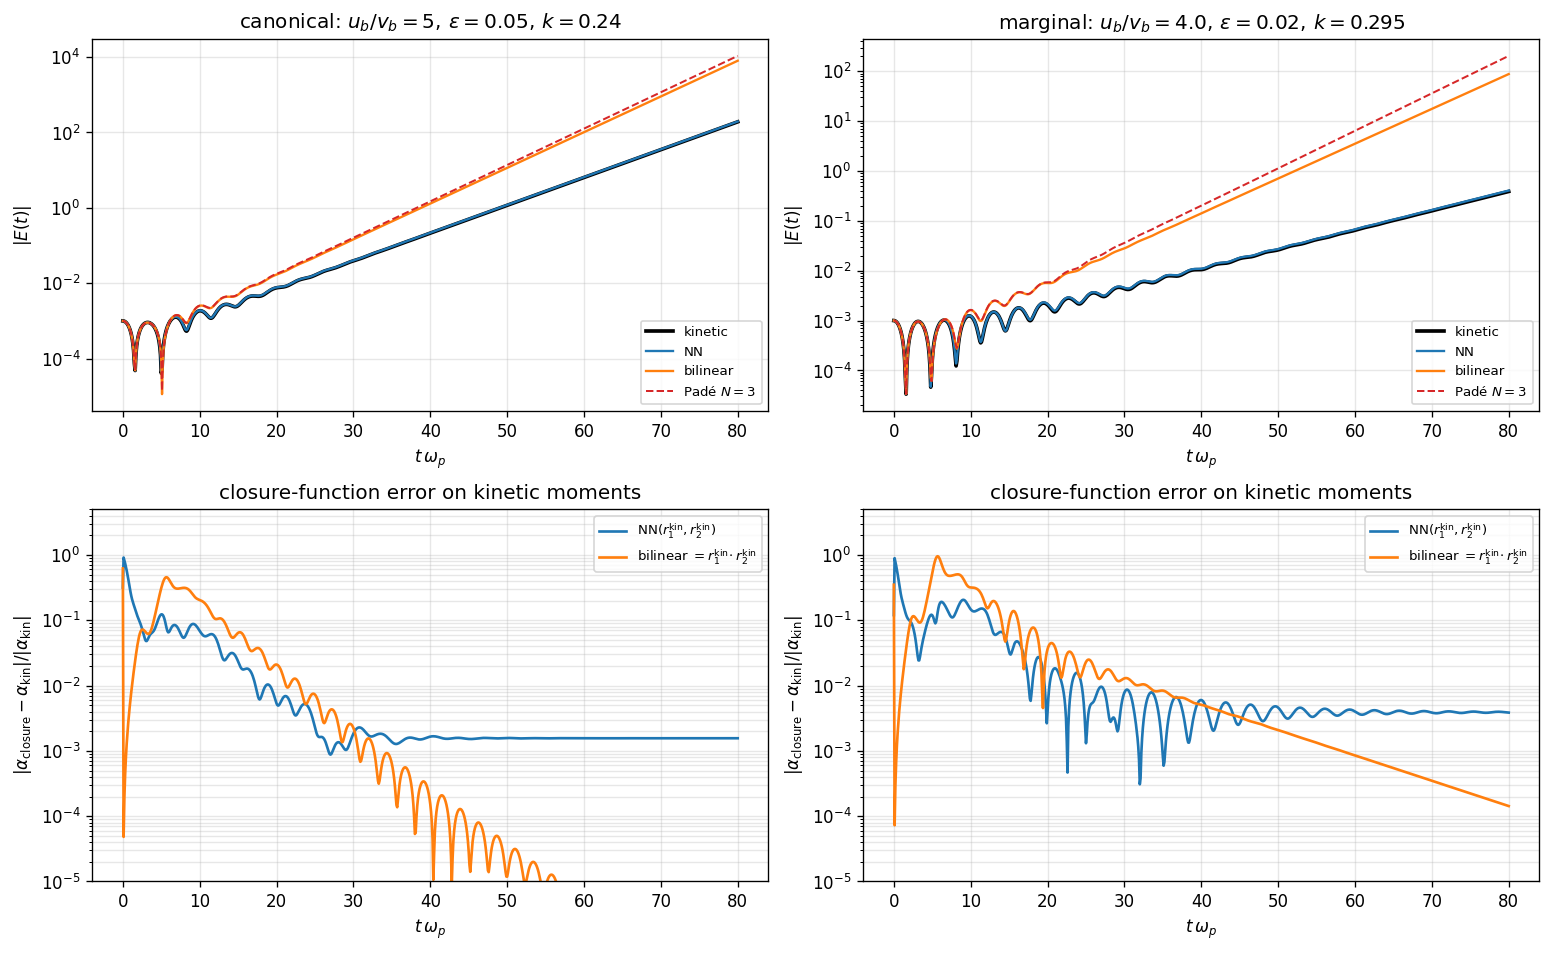
\includegraphics[width=\linewidth]{fig_offmanifold_diagnostic}
  \caption{Off-manifold diagnostic at canonical (left) and marginal
  (right) operating points. \emph{Top}: $|E(t)|$ for kinetic / NN /
  bilinear / Pad\'e under a generic $\delta E$ IC. Bilinear (orange)
  visibly tracks Pad\'e, not kinetic. \emph{Bottom}: closure-function
  error $|\alpha_{\rm closure} - \alpha_{\rm kin}| / |\alpha_{\rm kin}|$
  evaluated on the kinetic moments, isolating the closure function from
  trajectory feedback. NN: blue. Bilinear: orange. Early time
  ($t\lesssim 20$ canonical, $\lesssim 50$ marginal) the NN is one to
  two decades better than bilinear; once the unstable mode dominates,
  bilinear is exact and the NN plateaus at training residual.}
  \label{fig:offmanifold}
\end{figure}

\paragraph{Mechanism, in one line.} On the eigenmode manifold the
3-moment Maxwellian closure is bilinear and exact. The NN reproduces
that on the manifold and supplies a useful smooth extension off it ---
useful in the precise sense that it suppresses superposition cross-term
error at early time and lets the trajectory relax onto the manifold.
Linear closures (Pad\'e/HP) miss both the on-manifold and the
off-manifold structure; bilinear gets the on-manifold structure but
fails on the off-manifold extension; the NN gets both.

% =====================================================================
\section{Extension to the \texorpdfstring{$N=2$}{N=2} even-moment closure}
\label{sec:n2}

The analysis in Sections \ref{sec:results}--\ref{sec:interp} focused
on the $N=3$ closure: predicting $U_3$ from $(U_0,U_1,U_2)$.  We now
examine the $N=2$ level, where the closure target is $U_2$ from
$(U_0,U_1)$.

\paragraph{System and exact per-mode formula.}
Truncating at two beam moments gives the four-dimensional state
$y=(u,E,U_0,U_1)$ per Fourier mode $k$, with
$\partial_t U_1 = -ik\ub U_1 - ik U_2 + M_0 E$ and $M_0=1$.
On a single eigenmode the $n=0$ recurrence gives $U_1=\xib U_0$
(zero-RHS since $M_{-1}=0$), so $r_1\equiv U_1/U_0=\xib$
\emph{exactly}.  The $n=1$ step has nonzero source $M_0\Phih$ and
produces
\begin{equation}\label{eq:beta}
  \beta(\xib) \equiv \frac{U_2}{U_0}
               = \xib^2 - \frac{1}{Z'(\xib)}.
\end{equation}
Because $r_1=\xib$ the inference map is trivial, and the
\emph{direct-$\beta$} closure $U_2=U_0\,\beta(U_1/U_0)$ is
simultaneously the exact on-mode formula and the natural off-manifold
extension.

\paragraph{Structural contrast with $N=3$.}
At $N=3$ the $n=2$ recurrence has zero RHS ($M_1=0$), giving
$U_3=r_1 r_2 U_0$: the bilinear identity $\alpha=r_1r_2$
(Section~\ref{sec:bilinear}).  That identity is exact on eigenmode but
produces $O(1)$ cross-term errors off it, motivating the NN.  At
$N=2$ no bilinear identity exists ($M_0\neq0$), but the inference map
is trivial and the exact $\beta$ is already off-manifold-smooth: as
the Langmuir mode grows to dominate, $r_1\to\xib^{\rm kin}$ and
$\beta(r_1)\to\beta(\xib^{\rm kin})$ exactly.
Table~\ref{tab:structure} summarises the contrast.

\begin{table}[H]
\centering
\caption{Structural comparison of $N=2$ and $N=3$ Maxwellian-beam closures.}
\label{tab:structure}
\begin{tabular}{lll}
\toprule
 & $N=3$ ($U_3$, odd) & $N=2$ ($U_2$, even) \\
\midrule
Exact per-mode formula & $\alpha = \xib^3 - \xib/Z'(\xib)$ &
  $\beta = \xib^2 - 1/Z'(\xib)$ \\
Zero-parameter identity & $\alpha = r_1 r_2$ (bilinear) & none \\
NN input dimension & 4 reals & 2 reals \\
Inference ($r\to\xib$) & non-trivial & trivial: $r_1=\xib$ \\
Off-manifold & cross-terms $O(1)$; NN needed &
  smooth; exact formula sufficient \\
\bottomrule
\end{tabular}
\end{table}

\paragraph{Pad\'{e} $N=2$.}
A linear closure $U_2=a_0U_0+a_1U_1$ Taylor-matched at
$\xib\to\infty$ gives $\beta_{\rm Pad\acute{e}}(\xib)=a_0+a_1\xib$
with $a_0=-0.282$, $a_1=0.500i$---a poor approximation to the
nonlinear exact $\beta$ (Figure~\ref{fig:u2response}).

\begin{figure}[H]
  \centering
  
\includegraphics[width=\linewidth]{fig_u2_response}
  \caption{Left: kinetic response $-Z'(\xib)$ (solid) vs.\ Pad\'{e}
  rational (dashed) along real $\xib$.  Right: exact $\beta(\xib)$
  (Re solid / Im dotted) vs.\ Pad\'{e}-implied linear $\beta$
  (Re dashed / Im dash-dot).  The linear $\beta$ does not approximate
  the nonlinear exact $\beta$ for $|\xib|>0.5$.}
  \label{fig:u2response}
\end{figure}

\paragraph{Dispersion.}
Table~\ref{tab:disp_u2} gives $\gamma_{\max}$ overshoot at four
operating points.  Direct-$\beta$ recovers the kinetic rate to
numerical precision everywhere; Pad\'{e} $N=2$ overshoots by $+57\%$
at the canonical point and $+177\%$ near the marginal corner.

\begin{table}[H]
\centering
\caption{$\gamma_{\max}$ relative overshoot vs.\ kinetic, $N=2$ closures.}
\label{tab:disp_u2}
\begin{tabular}{ccrrr}
\toprule
$\ub/\vb$ & $\varepsilon$ & $\gamma_{\rm kin}$ &
  Pad\'{e} $N=2$ & Direct $\beta$ \\
\midrule
5.0 & 0.05 & $+0.17028$ & $+57\%$ & $0.00\%$ \\
5.0 & 0.20 & $+0.28919$ & $+28\%$ & $0.00\%$ \\
8.0 & 0.05 & $+0.19991$ & $+23\%$ & $0.00\%$ \\
3.0 & 0.05 & $+0.11254$ & $+177\%$ & $0.00\%$ \\
\bottomrule
\end{tabular}
\end{table}

\paragraph{Time-domain and off-manifold performance.}
Figure~\ref{fig:u2td} shows that direct-$\beta$ tracks the kinetic
reference to within numerical precision under both a
Langmuir-projected and a generic $\delta E$ IC, while Pad\'{e} $N=2$
diverges immediately owing to its $+55\%$ growth-rate error.
The off-manifold diagnostic (Figure~\ref{fig:u2offmfld}) shows that
Pad\'{e} $N=2$ plateaus at $\sim\!100$--$200\%$ closure error for
all time; direct-$\beta$ has a $\sim\!10\%$ transient during the
multi-mode phase ($t\lesssim10$) and then decays to $<\!10^{-5}$
as the Langmuir mode dominates and $r_1\to\xib^{\rm kin}$.

\begin{figure}[H]
  \centering
  
\includegraphics[width=\linewidth]{fig_u2_time_domain}
  \caption{$|E(t)|$ at the canonical point $(\ub/\vb,\varepsilon,k)=
  (5,0.05,0.24)$ for kinetic (black), Pad\'{e} $N=2$ (blue dashed),
  and direct-$\beta$ (orange) under a Langmuir-projected IC (left) and
  a generic $\delta E$ IC (right).  Fitted growth rates: kinetic
  $+0.170$, Pad\'{e} $+0.265$, direct-$\beta$ $+0.170$.}
  \label{fig:u2td}
\end{figure}

\begin{figure}[H]
  \centering
  
\includegraphics[width=0.85\linewidth]{fig_u2_offmanifold}
  \caption{Top: $|E(t)|$ along the kinetic trajectory (generic $\delta E$
  IC).  Bottom: closure error
  $|\beta_{\rm cl}-\beta_{\rm kin}|/|\beta_{\rm kin}|$
  evaluated at the kinetic moments.  Pad\'{e} $N=2$ (blue solid)
  plateaus at $\sim\!100$--$200\%$.  Direct-$\beta$ (orange dashed)
  peaks at $\sim\!10\%$ during the multi-mode transient and decays to
  $<\!10^{-5}$ once the Langmuir mode dominates.}
  \label{fig:u2offmfld}
\end{figure}

\paragraph{Parameter sweep.}
Over the same $(\ub/\vb,\varepsilon)$ grid as Section~\ref{sec:results}
(Figure~\ref{fig:u2sweep}), direct-$\beta$ stays within $\pm0.5\%$
everywhere; Pad\'{e} $N=2$ overshoot ranges from $+9\%$ (hot dense
beam) to $+800\%$ (cold sparse beam).

\begin{figure}[H]
  \centering
  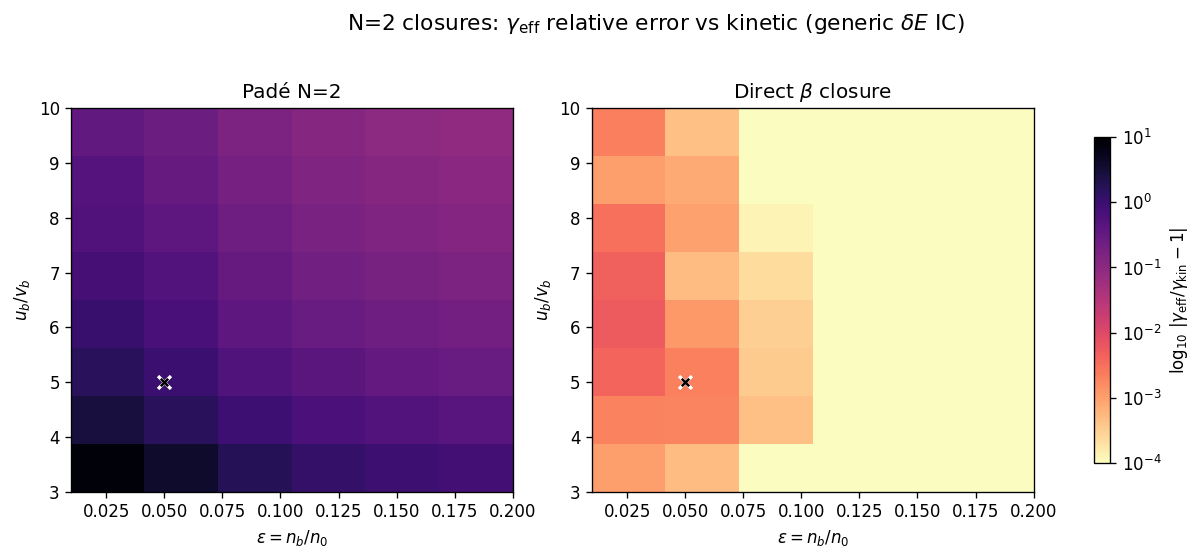
\includegraphics[width=\linewidth]{fig_u2_sweep}
  \caption{$\gamma_{\rm eff}$ relative error vs.\ kinetic on the
  $(\ub/\vb,\varepsilon)$ grid.  Left: Pad\'{e} $N=2$, uniformly in
  $10^0$--$10^1$.  Right: direct-$\beta$, $\lesssim\!10^{-3}$ for
  $\varepsilon\geq0.05$; the residual at the small-$\varepsilon$ edge
  is fitting noise, not closure error.}
  \label{fig:u2sweep}
\end{figure}

% =====================================================================
\section{Generalization: Landau damping on a single warm Maxwellian}
\label{sec:landau}

The trained closure $f_\theta(r_1, r_2) \to \alpha$ depends only on the
Maxwellian linear response: nothing in the training set references $\ub$,
$\varepsilon$, or $k$. So the same checkpoint should work for any
3-moment fluid system on a Maxwellian equilibrium, not just BoT. This
section confirms it by computing Landau damping of Langmuir waves on a
single warm Maxwellian -- a textbook benchmark unrelated to the BoT
instability.

\paragraph{Setup.} Strip the BoT system to a single warm species (drop
the cold bulk equations, set $\varepsilon = 1$, $\ub = 0$):
\begin{align*}
  \partial_t E   &= -U_1, \\
  \partial_t U_0 &= -ik U_1, \\
  \partial_t U_1 &= -ik U_2 + E   \quad (M_0 = 1), \\
  \partial_t U_2 &= -ik U_3       \quad (M_1 = 0,\;\text{closure}).
\end{align*}
The kinetic Langmuir dispersion in this normalization is $k^2 =
Z'(\omega/k)$, related to the standard $k\lambda_D$ convention by
$k_{\rm code} = \sqrt{2}\,k\lambda_D$ (BoT-paper variance is $1/2$, so
$v_{th} = 1/\sqrt{2}$).

\paragraph{Method.} For each $k\lambda_D$:
\begin{enumerate}\itemsep0pt
  \item Solve $k^2 = Z'(\omega/k)$ for the kinetic Langmuir mode (Newton from
        the Bohm-Gross seed) -- analytic ground truth.
  \item Project initial state onto the kinetic Langmuir eigenvector:
        $(E, U_0, U_1, U_2) = (U_1/i\omega,\, 1,\, \xi,\, \xi^2 - 1/Z'(\xi))$
        with $\xi = \omega_{\rm kin}/k$.
  \item Integrate the NN-closed and Pad\'e-closed fluid systems in time,
        fit $(\omega_r, \gamma)$ from late-time log-magnitude slope and
        real-part zero crossings.
\end{enumerate}
Projecting onto the kinetic eigenvector isolates the Langmuir mode --
without it, the fluid system's spurious closure eigenmodes (which exist
because there is no cold-bulk grounding) dominate the late-time signal.

\paragraph{Result.} Figure~\ref{fig:landau} shows
$(\omega_r, |\gamma|)(k\lambda_D)$ on $k\lambda_D \in [0.30, 0.60]$.

\begin{figure}[H]
  \centering
  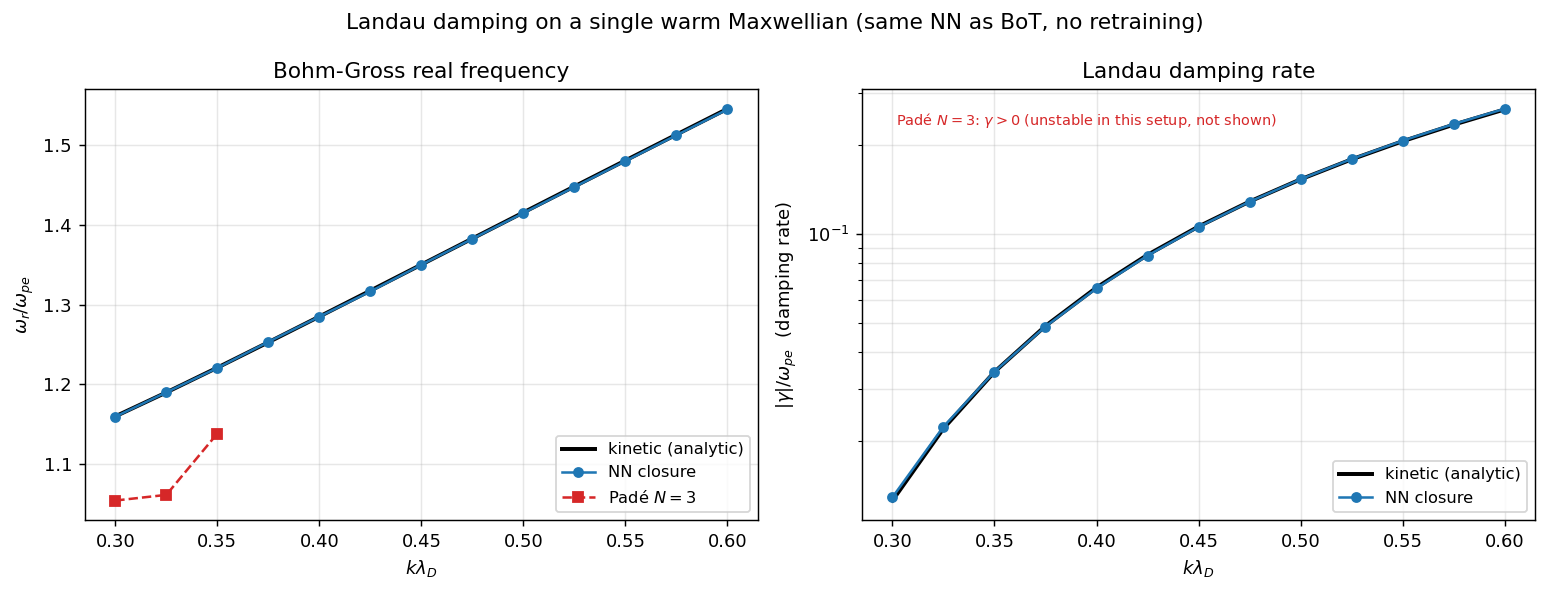
\includegraphics[width=\linewidth]{fig_landau_damping}
  \caption{Landau damping of Langmuir waves on a single warm Maxwellian,
  using the same NN checkpoint trained for BoT. \emph{Left}: Bohm-Gross
  real frequency. \emph{Right}: damping rate, log scale. The NN closure
  reproduces the kinetic ground truth (textbook values: $\gamma/\omega_{pe}
  = -0.0126$ at $k\lambda_D = 0.3$, $-0.1534$ at $k\lambda_D = 0.5$, etc.)
  to better than $1\%$ across the range. Pad\'e $N=3$ in this setup gives
  the wrong frequency and is unstable ($\gamma > 0$); not shown on the
  log-damping axis. See text.}
  \label{fig:landau}
\end{figure}

The NN curve overlays the kinetic curve in both panels. Representative
values:
\begin{center}\small
\begin{tabular}{lccc}
  \toprule
  $k\lambda_D$ & kinetic $\gamma/\omega_{pe}$ & NN $\gamma/\omega_{pe}$ &
  rel.\ error \\
  \midrule
  $0.30$ & $-0.0126$ & $-0.0129$ & $2.4\%$ \\
  $0.40$ & $-0.0661$ & $-0.0657$ & $0.6\%$ \\
  $0.50$ & $-0.1534$ & $-0.1535$ & $0.07\%$ \\
  $0.60$ & $-0.2641$ & $-0.2655$ & $0.5\%$ \\
  \bottomrule
\end{tabular}
\end{center}

\paragraph{Why Padé fails here.} The same Hunana-style Pad\'e closure
that gave $\sim 30\%$ overshoot on BoT $\gamma_{\rm eff}$ produces an
\emph{unstable} fluid system on the pure warm Maxwellian: $\gamma > 0$
even when initialized on the kinetic Langmuir eigenvector. This is a
known consequence of Taylor-matching closures in systems without
cold-fluid grounding; Hammett-Perkins-style frequency-axis filtering can
fix it but is a separate construction. The NN closure has no such
problem because the per-mode bilinear identity it learned
(Section~\ref{sec:bilinear}) gives the exact Langmuir eigenmode by
construction: the closed fluid system's Langmuir eigenvalue equation
reduces to $Z'(\omega/k) = k^2$ identically.

\paragraph{What this means.} The closure object stored in
\texttt{naive\_mlp.eqx} is a learned Maxwellian linear-response function.
It is reusable for any 3-moment fluid integrator with a Maxwellian
equilibrium and $\xib$ in the trained rectangle. BoT is one instance,
Landau damping on a warm Maxwellian is another, and the same logic
extends to ion-acoustic waves with adiabatic electrons, drift waves with
adiabatic species, or any model where the closure is "evaluate
$Z'$ of an effective $\xib$". A separate trained model is needed only
when the equilibrium is non-Maxwellian (kappa, flat-top, trapped
plateau) or when going beyond 3 moments (the per-mode identity at higher
order is not just a product because $M_2 \neq 0$).

\paragraph{Landau-damped BoT: Pad\'{e} structural failure.}
We return to the full BoT configuration but move into the regime where
the minority beam provides Landau \emph{damping} rather than
instability.  This requires $\ub<\omega_r/k$, so that
$\text{Im}(\xib)<0$ for the relevant mode.  Three test points are
$(\ub,k)=(2.0,\,0.30)$, $(1.5,\,0.40)$, $(1.0,\,0.50)$ with
$\varepsilon=0.05$.  The resulting $\xib$ values ($1.93{-}0.14i$ to
$1.25{-}0.34i$) lie well inside the training rectangle.

Figure~\ref{fig:u2ldamp} shows the growth rates from dispersion for all
$N=2$ closures.  Pad\'{e} $N=2$ predicts spurious instability ($\gamma>0$)
at every test point.  The reason is structural: the Taylor-series
approximant is anchored on the real $\xib$-axis and cannot represent
the Landau-pole contribution that lives in the lower half-plane
($\text{Im}(\xib)<0$).  The direct-$\beta$ and NN$(r_1)$ closures both
correctly predict negative $\gamma$ because they evaluate the Faddeeva
function at the actual complex $\xib$.  This failure is not a matter of
closure accuracy---it is a fundamental limitation of any polynomial or
rational approximation matched by Taylor expansion on the real axis.

\begin{figure}[H]
  \centering
  
\includegraphics[width=\linewidth]{fig_u2_landau_damping}
  \caption{Analytic growth rates $\gamma=\text{Im}(\omega)$ at three
  Landau-damped BoT test points (negative = damped).  Pad\'{e} $N=2$
  (blue) predicts positive $\gamma$ at every point, a qualitative failure.
  Direct-$\beta$ (orange) and NN$(r_1)$ (green) correctly predict
  negative $\gamma$.  Right panel: $\xib$ locations in the complex plane;
  all points lie within the training rectangle.}
  \label{fig:u2ldamp}
\end{figure}

\paragraph{Comparing $N=2$ and $N=3$ closures off eigenmode.}
To compare closures across both truncation levels under multi-mode
conditions, we integrate from a generic $\delta E$ IC at each
Landau-damped test point and compare to the kinetic ground truth.
To first establish a clean baseline, Figure~\ref{fig:ldamp_eig} shows
$|E(t)|$ under an eigenmode-projected IC (top row) and a generic
$\delta E$ IC (bottom row), for all available $N=2$ and $N=3$ closures.

\begin{figure}[H]
  \centering
  
\includegraphics[width=\linewidth]{fig_u2_landau_eigenmode}
  \caption{Top row: eigenmode-projected IC.  Direct-$\beta$ N=2 and
  direct-$\alpha$ N=3 (exact on eigenmode) decay cleanly along the
  reference slope $e^{\gamma_{\rm kin}t}$.  Both NNs also decay but
  level off at later times as approximation error accumulates.  The
  kinetic $N_v{=}96$ curve is nearly flat: $O(10^{-14})$ mixing with
  van~Kampen quasi-continuum modes dominates after $\sim\!10$ e-folds.
  Bottom row: generic $\delta E$ IC; kinetic (black) is ground truth.}
  \label{fig:ldamp_eig}
\end{figure}

Table~\ref{tab:offmfld} gives the mean relative error
$\bar\epsilon=\langle|E_{\rm cl}-E_{\rm kin}|/|E_{\rm kin}|\rangle$
over $t\in[5,30]$ for the generic-IC runs.  Four patterns stand out.
\emph{NN naive$(r_1,r_2)$ N=3 is the best or joint-best}: the second
input $r_2=\langle\beta(\xi)\rangle$ carries genuine off-eigenmode
information about the spread of $\xi$ across modes.
\emph{NN inference N=3 is the worst} (worse than even the
parameter-free direct-$\alpha$): the inference bottleneck forces a
single $\hat\xib$ inconsistent with multi-mode $r_1$ and $r_2$, and the
exact Faddeeva at the compromised $\hat\xib$ amplifies the error.
\emph{Direct-$\alpha$ N=3 is the second worst}: $\alpha$'s larger
curvature amplifies the Jensen error relative to $\beta$.
\emph{Direct-$\beta$ N=2 and NN$(r_1)$ N=2 are comparable}, as both
use only $r_1$.

\begin{table}[H]
\centering
\caption{Mean relative error vs.\ kinetic under generic $\delta E$ IC,
  $t\in[5,30]$.  ``Naive'' NN maps $(r_1,r_2)\to\alpha$ directly;
  ``Inference'' NN maps $(r_1,r_2)\to\hat\xib\to\alpha(\hat\xib)$.}
\label{tab:offmfld}
\begin{tabular}{lccccc}
\toprule
Case & Dir.\ $\beta$ N=2 & NN$(r_1)$ N=2 & Dir.\ $\alpha$ N=3 &
  NN naive N=3 & NN inf.\ N=3 \\
\midrule
$\ub=2.0$, $k=0.30$ & 0.24 & 0.24 & 0.37 & \textbf{0.13} & 0.42 \\
$\ub=1.5$, $k=0.40$ & 0.13 & 0.14 & 0.33 & \textbf{0.10} & 0.45 \\
$\ub=1.0$, $k=0.50$ & 0.12 & \textbf{0.10} & 0.44 & 0.11 & 0.50 \\
\bottomrule
\end{tabular}
\end{table}

% =====================================================================
\section{Extension to the $N=4$ hierarchy: Jensen error and superposition training}
\label{sec:n4}

The off-manifold diagnostic (Table~\ref{tab:offmfld}) shows that the naive
$N=3$ NN is the best available closure at that truncation level.  This section
asks whether adding one more moment ($U_3 \to U_4$ closure) allows the
systematic Jensen error to be eliminated by training.

\paragraph{Jensen error and degrees of freedom.}
For a two-mode beam state
$U_n = w_1 U_n^{(1)} + w_2 U_n^{(2)}$ the ideal closure is the
amplitude-weighted average
\begin{equation}
  \hat\alpha_4 = w_1\,\alpha_4(\xib^{(1)}) + w_2\,\alpha_4(\xib^{(2)}).
\end{equation}
Whether any NN can learn this depends on whether its inputs uniquely determine
$(\xib^{(1)},\xib^{(2)},w)\in\mathbb{C}^3$---six real unknowns.
At $N=3$, inputs $(r_1, r_2)$ provide only four real numbers:
\emph{underdetermined}.  No training data can teach a four-real-input closure
to be Jensen-free, because the mapping from two-mode state to inputs is not
injective.  At $N=4$, inputs $(r_1, r_2, r_3)$ provide six real numbers,
matching the six unknowns: the system is \emph{generically solvable}.  The
Jensen error is irreducible at $N=3$ and trainable at $N=4$.

\paragraph{The $N=4$ hierarchy.}
Extending by one moment gives state $y=(u,E,U_0,U_1,U_2,U_3)$ and closure
$U_4 = \alpha_4(\xib)\,U_0$.  The additional evolution equation is
\begin{equation}
  \partial_t U_3 = -ik\ub U_3 - ik U_4 + \tfrac{3}{2}\,E,
\end{equation}
where the source $3M_2 E = \tfrac{3}{2}E$ comes from the Maxwellian second
moment $M_2 = 1/2$.  Iterating the recurrence from $U_0 = Z'(\xib)$ gives the
exact per-mode closure ratio
\begin{equation}\label{eq:alpha4}
  \alpha_4(\xib) \;\equiv\; \frac{U_4}{U_0}
  \;=\; \xib^4 - \frac{\xib^2 + 3/2}{Z'(\xib)}.
\end{equation}
The three input ratios are $r_1 = \xib$, $r_2 = \beta(\xib)$
(equation~\ref{eq:beta}), $r_3 = \alpha(\xib)$ (equation~\ref{eq:alpha}),
giving a 6-real-input MLP $(64,64,64,64)$ that predicts $\alpha_4$ directly.

\paragraph{Superposition training.}
To make the NN Jensen-free, we augment the frequency-domain dataset with
multi-mode samples.  The combined training set has three equal components
($N = 16{,}384$ each):
\begin{enumerate}\itemsep0pt
  \item \emph{Single eigenmode}: $\xib$ uniform in the training rectangle
        (same as before).
  \item \emph{Complex-weight two-mode}: $\xib^{(1)}, \xib^{(2)}$ independently
        sampled in the rectangle; weight $w = a/(1+a)$ with
        $\log|a| \sim \mathrm{Uniform}(-1.5,1.5)$,
        $\arg a \sim \mathrm{Uniform}(0,2\pi)$.
        Pairs with $|\xib^{(1)}-\xib^{(2)}|<0.15$ or $|\alpha_4|>50$ are rejected.
  \item \emph{Chord (real-weight two-mode)}: same mode pairs with real
        $s\in(0.02,0.98)$ uniform.  This component is measure-zero in the
        complex-weight distribution and must be included explicitly so the NN
        sees the chord target during training.
\end{enumerate}
Total $\approx 50{,}000$ samples; Adam cosine $3\!\times\!10^{-3}\to10^{-5}$,
$30{,}000$ steps.

\paragraph{Chord test and results.}
Figure~\ref{fig:n4chord} shows the chord test: fix a mode pair
$(\xib^{(1)},\xib^{(2)})$, vary the real mixing weight $s\in[0,1]$, and
compare each closure's output to the target chord
$\alpha_4^{\rm chord}(s) = (1-s)\,\alpha_4(\xib^{(1)}) + s\,\alpha_4(\xib^{(2)})$.
All single-eigenmode-trained closures---including the analytic
direct-$\alpha_4$, which evaluates \eqref{eq:alpha4} at $r_1$ alone---trace
curves that deviate from the chord because they were never exposed to
superposition states.  The superposition-trained NN tracks the chord closely.

\begin{figure}[H]
  \centering
  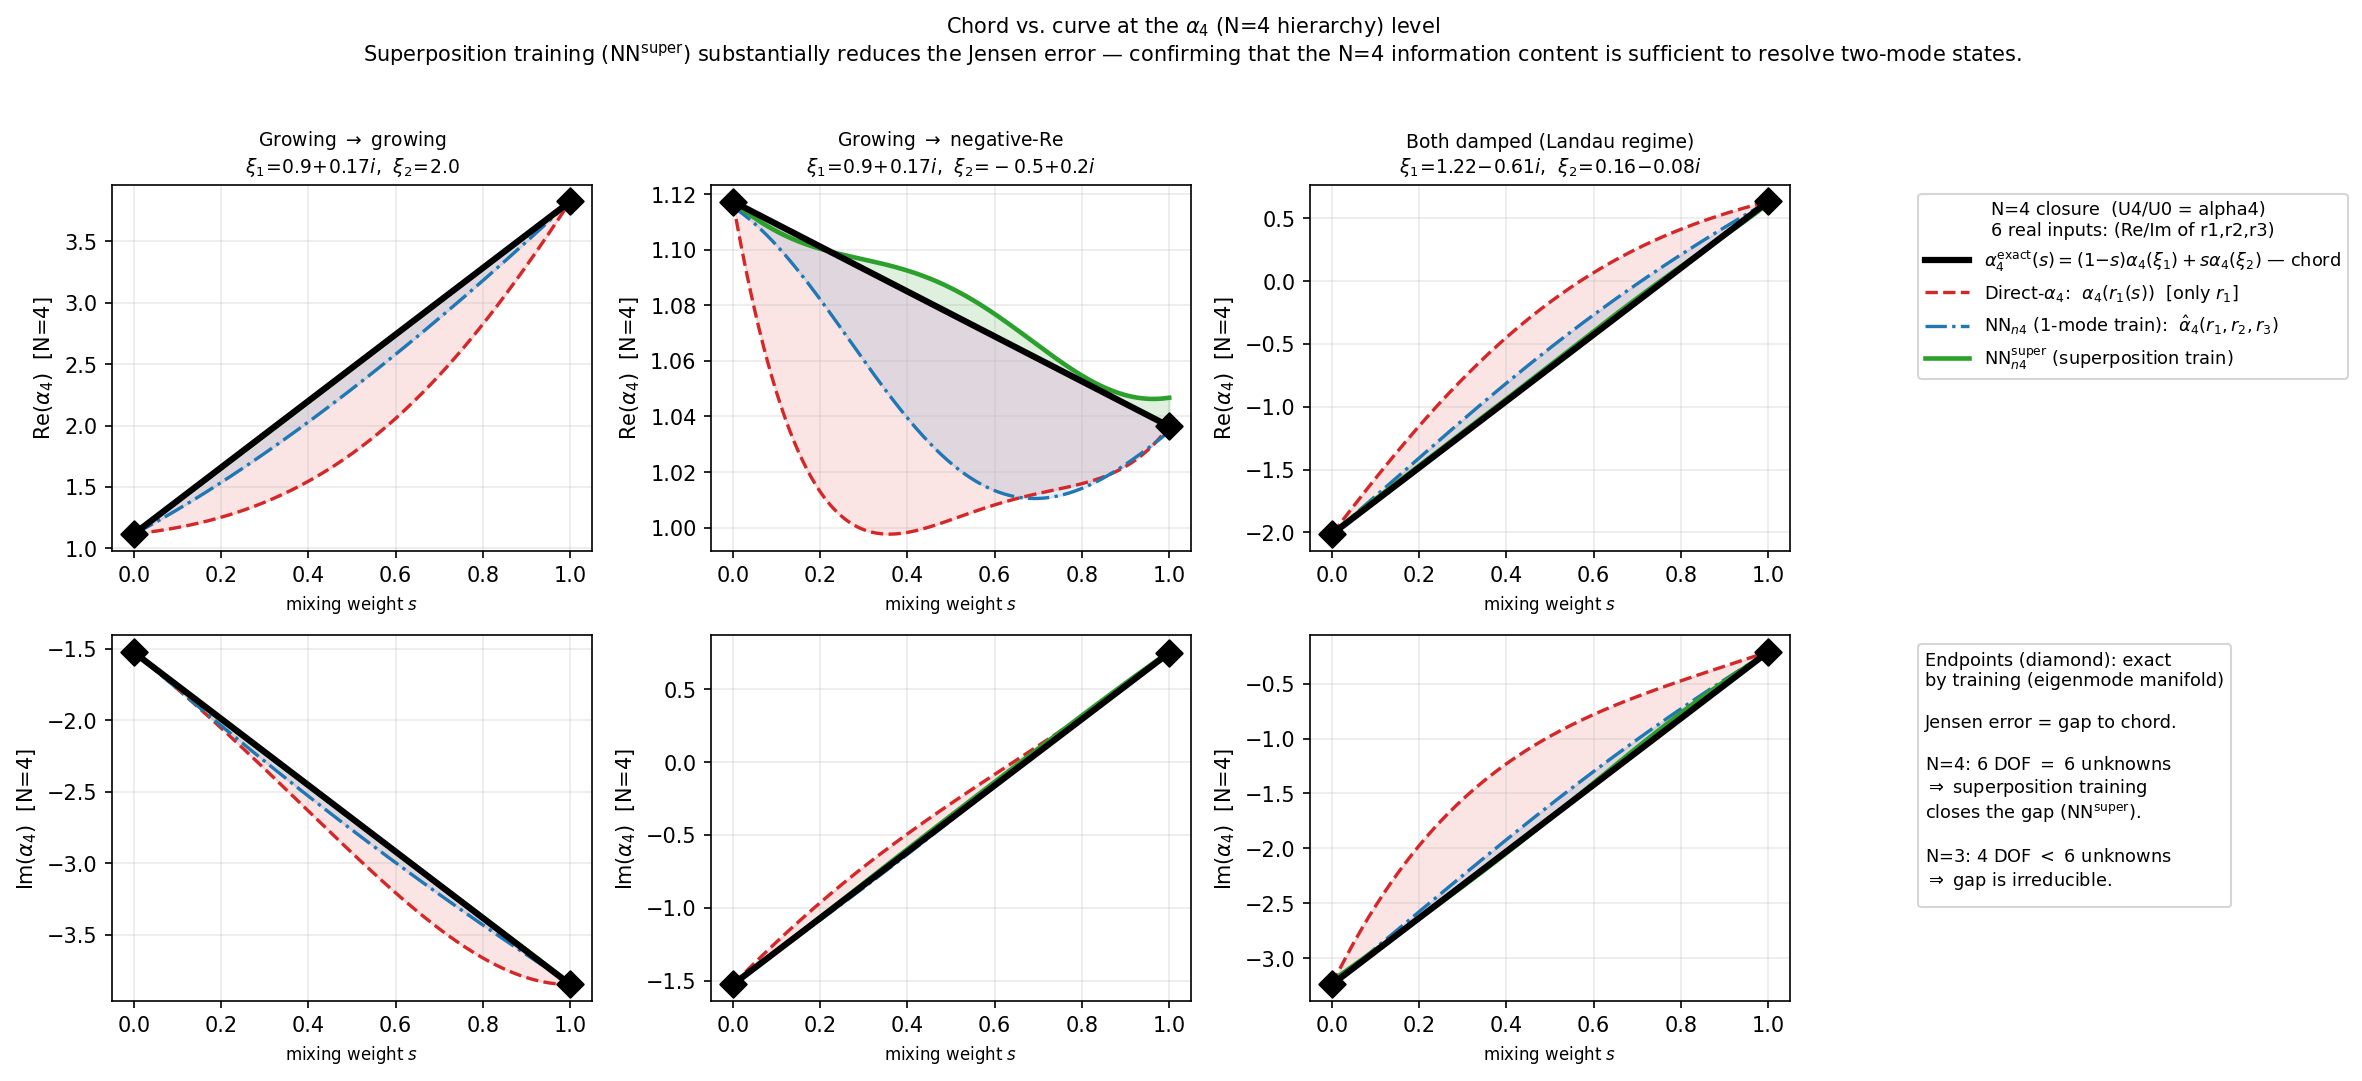
\includegraphics[width=\linewidth]{fig_n4_chord}
  \caption{Chord test for the $N=4$ closure across three mode pairs (columns;
  real part top row, imaginary part bottom row).
  Black: ideal chord target.
  Red dashed: direct-$\alpha_4$ (evaluates~\eqref{eq:alpha4} at $r_1$ only;
  also develops spurious instability in time-domain at $t\gtrsim40$).
  Blue dash-dot: $N=4$ NN, single-eigenmode training.
  Green solid: $N=4$ NN, superposition training.}
  \label{fig:n4chord}
\end{figure}

Table~\ref{tab:n4chord} quantifies the maximum relative chord error
$\max_s|\hat\alpha_4(s)-\alpha_4^{\rm chord}(s)|/|\alpha_4^{\rm chord}(s)|$.

\begin{table}[H]
\centering
\caption{Maximum relative chord error for the $N=4$ NN before and after
superposition training.}
\label{tab:n4chord}
\begin{tabular}{lcc}
\toprule
Closure & Growing--growing & Landau-damped \\
\midrule
$N=4$ NN, single-mode training   & $5.8\%$    & $16.8\%$   \\
$N=4$ NN, superposition training & $0.4\%$    & $6.4\%$    \\
Reduction                        & $15\times$ & $2.6\times$ \\
\bottomrule
\end{tabular}
\end{table}

The $15\times$ improvement on growing--growing pairs confirms the DOF
prediction: $N=4$ has sufficient information content to learn a Jensen-free
closure.  The smaller improvement on Landau-damped pairs reflects a genuine
physical limitation---rapid Landau decay requires phase mixing of van~Kampen
continuum modes, which is inherently kinetic and cannot be reproduced by any
finite-moment fluid closure regardless of training.  The residual Landau chord
error at $N=4$ is therefore not a deficiency of the training scheme.

\paragraph{Stability.}
The analytic direct-$\alpha_4$ closure evaluates~\eqref{eq:alpha4} at $r_1$
alone.  In time-domain integration it develops a spurious exponentially growing
mode at $t\approx 40$, a pathology absent in the exact kinetic system that the
per-mode formula does not suppress.  The $N=4$ NN closure, whose off-manifold
behavior is constrained by training data, remains stable past $t=80$.

% =====================================================================
\section{Discussion}

\paragraph{Where the win comes from.} Both wins --- accuracy and cost ---
trace to the same observation: the closure problem is parameterised by a
single complex variable $\xib$. Simulation training generates
$(\mathrm{ratios}, \alpha)$ pairs via the parameterisation $(\ub/\vb,
\varepsilon, k, \mathrm{IC}, t) \mapsto \xib$, which is many-to-few and
covers only a 1-parameter family of $\xib$ values (the unstable
eigenmode), at the cost of a kinetic integration per operating point.
Frequency-domain training generates the same pairs via the identity
$\xib \mapsto (\mathrm{ratios}, \alpha)$, which is one-to-one, covers
whatever subset of $\mathbb{C}$ we choose, and reduces dataset generation
to a Faddeeva evaluation. The 2D rectangle is the natural, dense,
problem-agnostic training distribution because moment ratios from the 5-d
fluid system's other (damped) eigenmodes also land in this rectangle.

The sim-trained closure is not bad --- $\sim\!10\%$ on $\gamma_{\rm eff}$
across most of the grid is a real improvement over Pad\'e. The honest
framing is that the closed-form approach is strictly better on every axis
that matters: tighter error (two decades), cheaper data (two orders of
magnitude), problem-agnostic (no operating-point sweep), and trivially
re-trained when the operating regime shifts.

The same logic applies to other moment closures whose linear-response
function is one-parameter (drift--kinetic with one resonance, weakly
collisional fluid models on a Maxwellian background): if there is an
analytical $\xib \mapsto \alpha$ map, frequency-domain sampling is
strictly better than simulation sampling at fixed dataset size.

\paragraph{What is not solved.} The training is entirely linear-physics:
$\alpha(\xib)$ is derived assuming the beam perturbation is linear about
the Maxwellian $f_{b0}$. Capturing trapping, plateau formation, and
saturated BoT requires kinetic training data and is outside this scope.
The $\xib$-rectangle covers the unstable BoT regime by construction; the
marginal corner $(\ub/\vb \lesssim 3, \varepsilon \lesssim 0.02)$ pushes
$\xib$ to the rectangle's lower edge and shows mild degradation.

\paragraph{Relation to the Pad\'e / Hunana hierarchy.} Hunana et al.\
(2019) construct rational closures of $Z'(\zeta)$ up to 8 poles and prove
asymptotic convergence with increasing order. The NN closure trades the
rational-order ceiling for NN expressivity; the present work shows the
fluid response problem itself isn't the obstacle --- training-data design
is.

\paragraph{Inference vs.\ naive NN architecture.}
At $N=3$, two distinct NN parameterisations have been tested.  The
\emph{inference} architecture maps $(r_1,r_2)\to\hat\xib$ and then
evaluates $\alpha(\hat\xib)$ via the exact Faddeeva function.  The
\emph{naive} architecture maps $(r_1,r_2)\to\alpha$ directly.

On the single-eigenmode manifold, both are equivalent by construction:
$(r_1,r_2)$ determines $\xib$ uniquely, so the inversion is exact and
the two designs converge to the same prediction.  Off eigenmode---as
quantified in Table~\ref{tab:offmfld}---they diverge sharply.  The
inference NN is the \emph{worst} performer (42--50\% mean relative
error), worse than the parameter-free direct-$\alpha$.  The reason is
structural: in a multi-mode state, $r_1=\langle\xi\rangle$ and
$r_2=\langle\beta(\xi)\rangle$ cannot simultaneously be consistent with
any single $\hat\xib$, so the NN settles on a compromised value, and the
exact Faddeeva applied there amplifies rather than corrects the error.
The inference design embeds the wrong physical assumption---that the beam
is always in a single eigenmode---directly into the architecture.

The naive NN carries no such assumption.  Its direct $(r_1,r_2)\to\alpha$
map learns a smooth, non-multiplicative function that implicitly
approximates $\langle\alpha(\xi)\rangle$ from partial moment information,
without committing to any single-resonance picture.  This makes it the
most robust closure when multiple modes are simultaneously present, which
is the generic situation in a fluid simulation.

The practical recommendation is therefore: \emph{train the NN as a direct
map from moment ratios to the closure coefficient, not as an inference
engine for an intermediate physical parameter.}  The exact Faddeeva is
beneficial only when $\xib$ is known exactly; when it must itself be
inferred from multi-mode moment data, the inversion error propagates
nonlinearly.

\paragraph{Even-moment closures.}
As shown in Section~\ref{sec:n2}, the $N=2$ closure illustrates the
complementary case where no NN is needed at all: the inference map is
trivial ($r_1=\xib$), the exact $\beta$ is analytically available, and
its off-manifold behavior is already superior to any linear approximation.
The interesting NN problem arises at higher levels where the per-mode
formula involves multiple Maxwellian moments and the Jensen error reappears.
Section~\ref{sec:n4} shows that the $N=4$ level is the first at which the
Jensen error is information-theoretically trainable: the additional
input $r_3 = \alpha(\xib)$ supplies the two real degrees of freedom
needed to resolve a two-mode superposition, and superposition training
achieves a $15\times$ reduction in growing-mode chord error.

\section*{Code}

The accompanying \texttt{bot/} package implements all figures and runs:
\begin{itemize}\itemsep0pt
  \item \texttt{closures/pade.py} --- Pad\'e closure coefficients and the
    closed fluid response.
  \item \texttt{closures/naive\_nn.py} --- NN closure (MLP $\to \alpha$),
    closed-form $\xib$-sampling dataset, training.
  \item \texttt{closures/n4\_nn.py} --- $N=4$ NN closure
    ($\mathrm{MLP}_{N=4} : (r_1,r_2,r_3) \to \alpha_4$), single-mode
    dataset, three-component superposition dataset, and training;
    checkpoints \texttt{runs/n4\_nn.eqx} (single-mode) and
    \texttt{runs/n4\_nn\_super.eqx} (superposition).
  \item \texttt{closures/u2.py} --- $\beta(\xib)$ exact formula, MLP$_{u2}$
    (2-input NN for $\beta$), training utilities.
  \item \texttt{train\_simdata.py} --- sim-data NN training (single- and
    broad-sweep).
  \item \texttt{kinetic.py}, \texttt{fluid.py} --- kinetic ground truth and
    two-fluid eigenvalue system.
  \item \texttt{closed\_loop.py} --- time-domain integration for all
    closures; eigenmode IC helpers for $N=2$, $N=3$, $N=4$, and kinetic;
    direct-$\alpha_4$ and NN$_{N=4}$ time-domain integrators.
  \item \texttt{sweep.py}, \texttt{sweep\_timedomain.py} --- 2D parameter
    scans.
  \item \texttt{figures.py} --- $N=3$ plots and the $N=4$ chord figure
    (\texttt{fig\_n4\_chord}).
  \item \texttt{figures\_u2.py} --- $N=2$, Landau damping, and $N=2$/$N=3$
    comparison plots; updated to include both $N=4$ model variants in the
    two-mode Landau-damped time-domain panel.
\end{itemize}

\end{document}
